\chapter{System Architecture}
\label{sec:arch}

SiliconScribe is a three-tier system (Figure~\ref{fig:arch}): a React frontend, a
FastAPI backend, and a local EDA toolchain (Icarus Verilog, Yosys and OpenSTA). The backend is the only component that
holds credentials and the only component that executes subprocesses. The frontend
communicates over HTTP and Server-Sent Events (SSE), so the diagnosis timeline is
streamed while the simulation runs.


\section{Frontend}
The React single-page application consists of a prompt panel (with example prompts,
frequency hint, and model selector), two CodeMirror editors for RTL and testbench,
a workspace pane with \emph{Design / Results / Test cases / Waveform / Schematic}
tabs, an agent chat timeline fed by SSE, and a project-history drawer. The sidebar
holds the model menu (Figure~\ref{fig:home}): the model for the run, a
``Testbench written by'' select for an optional separate testbench model, and a
``Review the specification before generating'' checkbox that opens an editable
specification panel before any code is generated. The Results tab shows the
verdict, which model wrote the design, the testbench strength, the timing and area
estimate, the measured toggle coverage and any verification warning. The waveform viewer is a native
SVG renderer with a time ruler, hexadecimal bus values, zoom, and reset. It avoids
an external GTKWave dependency.

\begin{figure}[H]
\centering
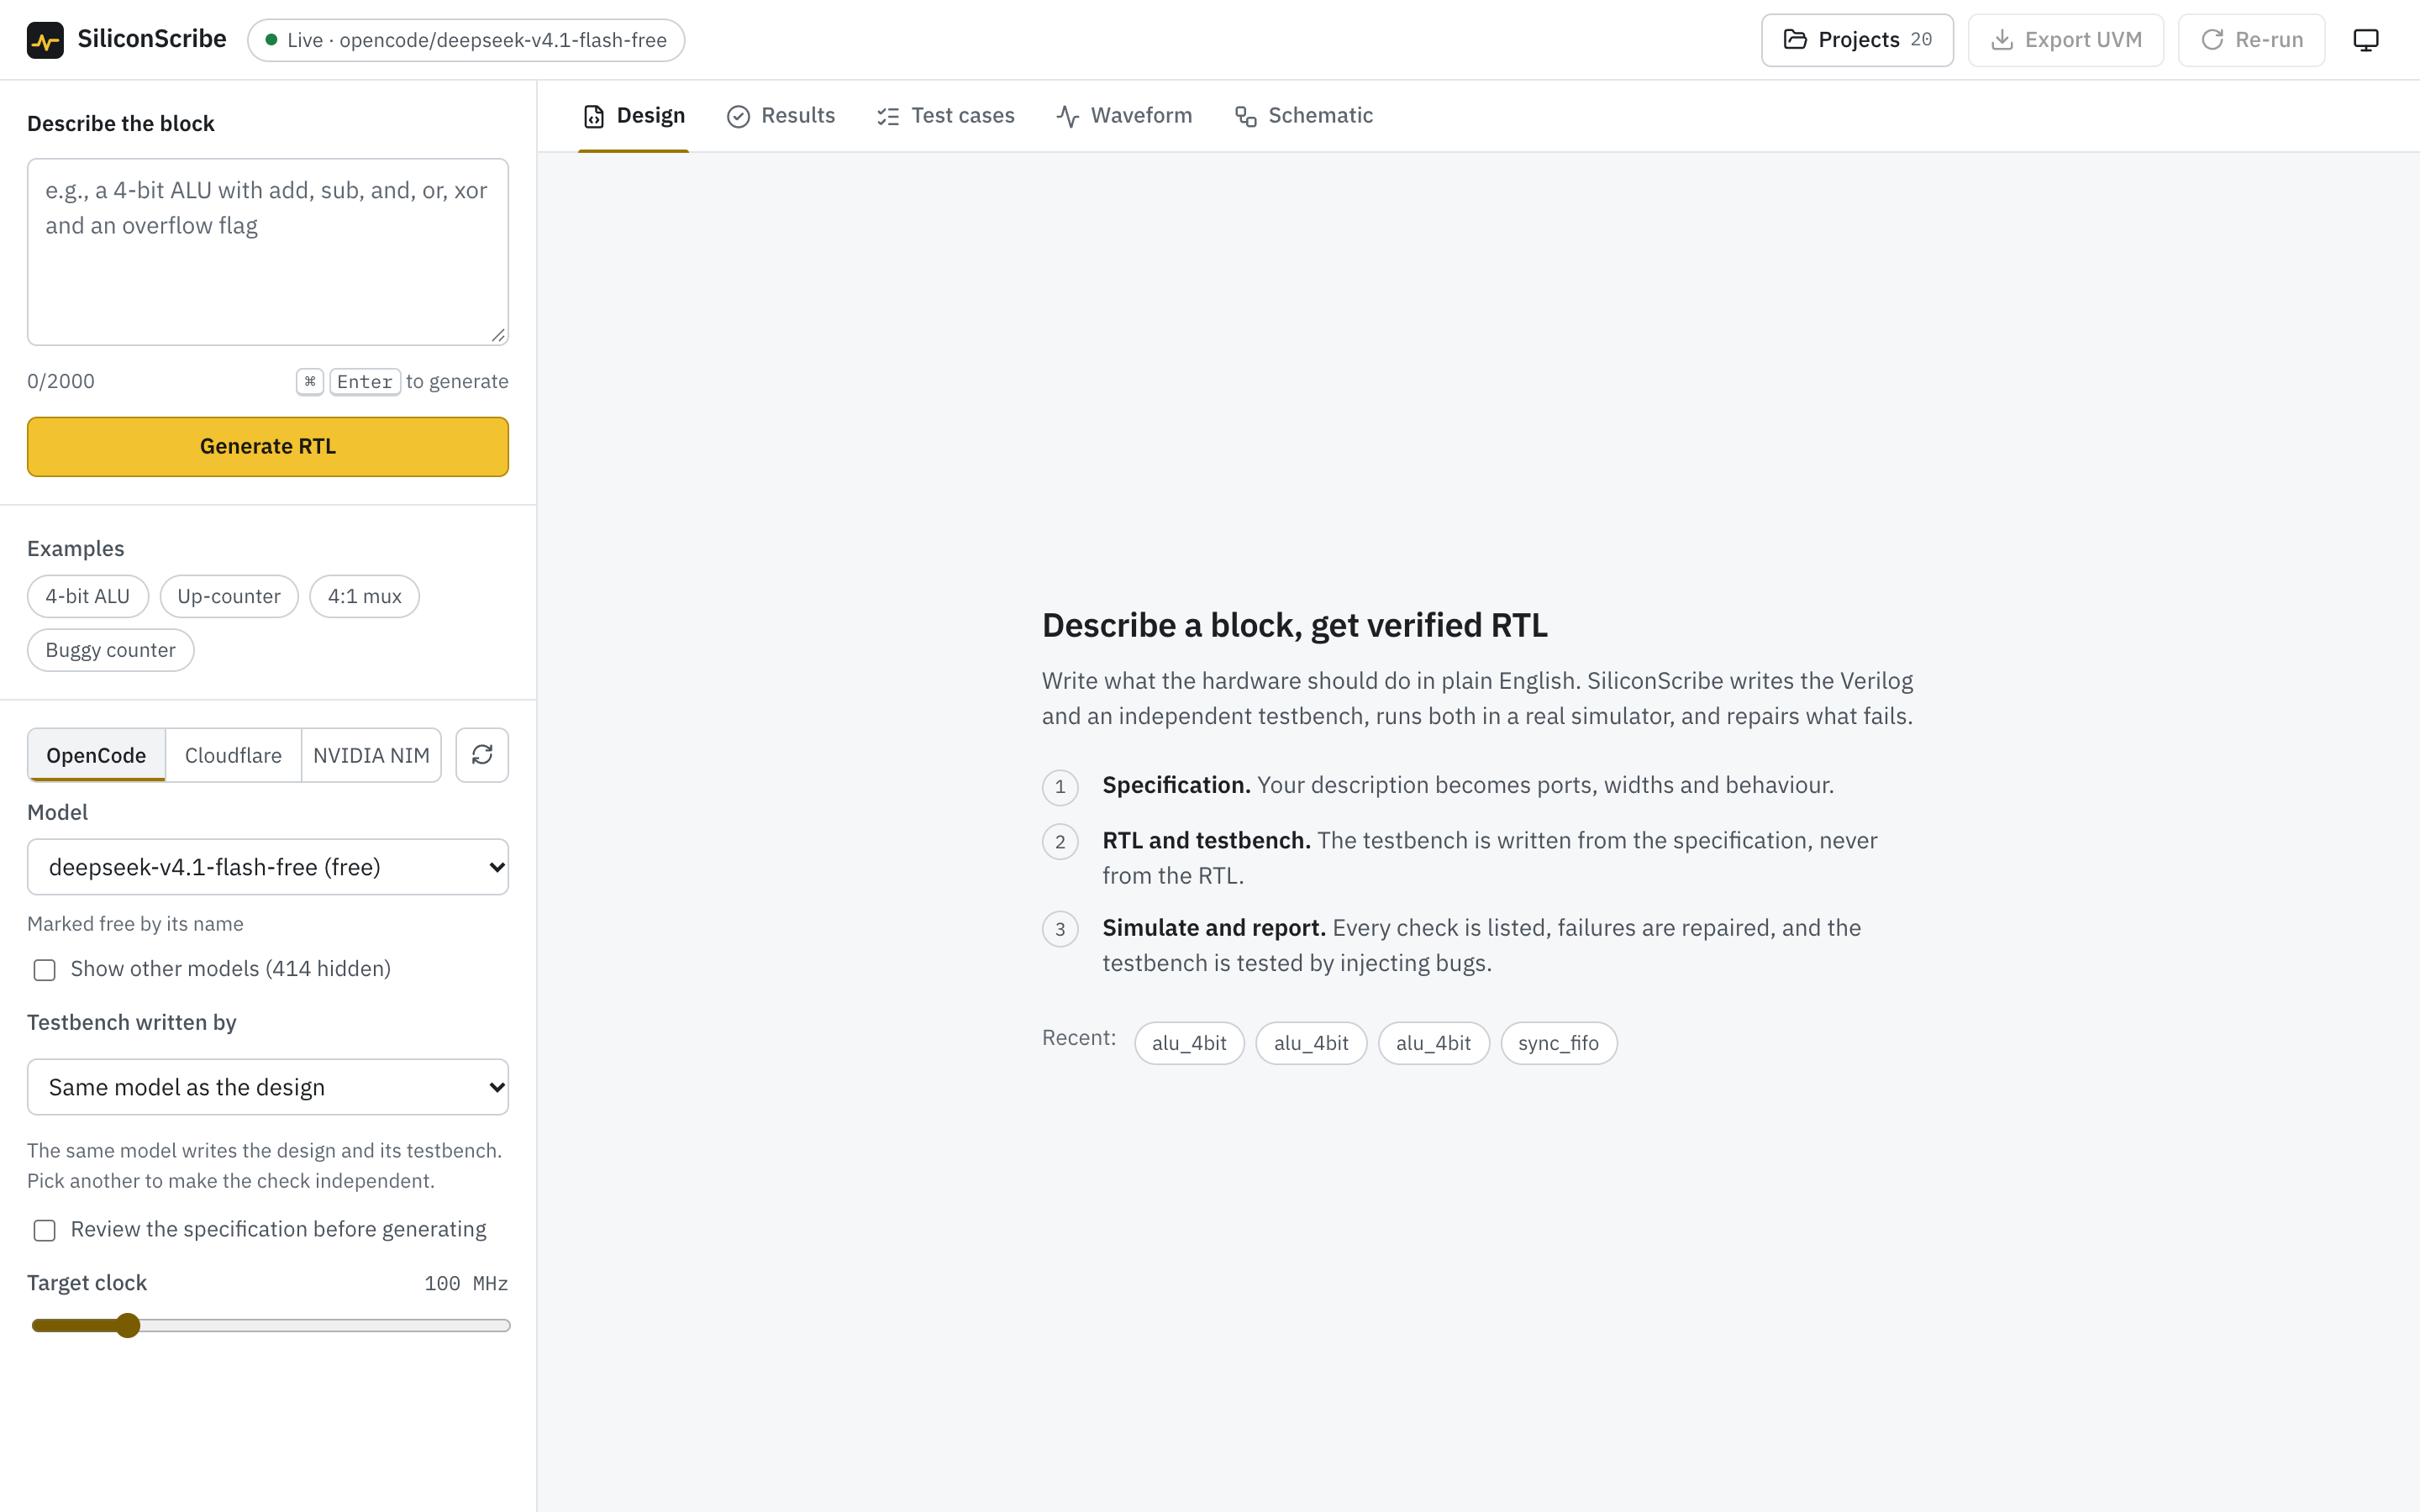
\includegraphics[width=0.85\textwidth]{figures/s01_welcome.png}
\caption{Start screen of the current build. The sidebar (left) holds the prompt box, example prompts, the per-run model menu with its OpenCode, Cloudflare and NVIDIA NIM tabs, the ``Testbench written by'' select, the ``Review the specification before generating'' checkbox and the target clock; the workspace (right) shows the Design / Results / Test cases / Waveform / Schematic tabs and a three-step explanation. The badge at the top names the live model.}
\label{fig:home}
\end{figure}

\section{Backend}
The FastAPI service exposes the endpoints of Table~\ref{tab:api}: the
full pipeline as a Server-Sent Events stream or as one JSON reply,
specification parsing, simulation, synthesis, timing, the model list, saved
projects, UVM export, and health/status endpoints. Each
design runs in an isolated workspace directory named by a 32-character design ID;
paths are validated against a strict regular expression before any file operation. Generated Verilog is additionally screened by a sandbox policy (Section~\ref{sec:sandbox}) before it is compiled.
Rate limiting is per client IP. SQLite stores project metadata and the latest
result so the history drawer can reload a design.

\section{Provider Isolation and Model Routing}
\label{sec:routing}
All model calls go through one interface in \code{llm_service.py}. Only the backend
holds credentials, and it reads them only from the git-ignored \code{backend/.env}
file, never from the web page. The default provider is chosen from the environment:
\code{OFFLINE_MODE} forces the curated offline provider; \code{LLM_PROVIDER=opencode-app}
drives the user's installed OpenCode app through its command-line interface (each
call runs in a fresh empty temporary directory with the read-only \code{plan} agent);
otherwise an OpenCode Zen, NVIDIA or OpenAI-compatible key selects that endpoint.
Per-stage overrides such as \code{LLM_MODEL_TESTBENCH} are still read from the
environment, but a model picked in the interface overrides them.

On top of this default, the user picks a model for each run from the model menu
(Figure~\ref{fig:home}), which merges three live catalogues
(Table~\ref{tab:routing}). The backend routes each request by the form of the model
identifier: \code{@cf/...} goes to Cloudflare Workers AI, \code{nim/...} goes to
NVIDIA NIM, and anything else goes to the configured provider (normally the OpenCode
app). GitHub Copilot appears only through OpenCode, as \code{github-copilot/auto}:
on the student plan GitHub picks the model and does not disclose which one, so the
result cannot name it.

\begin{table}[H]
\centering
\caption{Model sources in the per-run model menu (counts as read on 19 November 2026).}
\label{tab:routing}
\footnotesize
\begin{tabularx}{\textwidth}{@{}p{2.3cm}X p{3.3cm} p{3.7cm}@{}}
\toprule
\textbf{Source} & \textbf{How the list is obtained} & \textbf{Identifier form} & \textbf{Set up by} \\
\midrule
OpenCode app & \code{opencode models}, read live and cached; about 460 models, those whose name says free first, the rest behind ``Show other models'' & \code{opencode/<name>} & installed, signed-in OpenCode app \\
GitHub Copilot & listed by the OpenCode app & \code{github-copilot/auto} only & Copilot plan inside OpenCode \\
Cloudflare Workers AI & live catalogue through its OpenAI-compatible endpoint; 40 text models on the account & \code{@cf/<org>/<model>} & \code{CLOUDFLARE_ACCOUNT_ID}, \code{CLOUDFLARE_API_TOKEN} \\
NVIDIA NIM & live catalogue of the hosted API; 15 chat models & \code{nim/<org>/<model>} & \code{NVIDIA_NIM_API_KEY} \\
\bottomrule
\end{tabularx}
\end{table}

A model identifier comes from the browser and ends up as a subprocess argument or in a
URL, so it is checked against a strict pattern (no leading dash, no spaces or shell
characters) before it is used. A model the user chose that fails is reported in plain
words and is never replaced by the scripted demo; only the configured default keeps
the labelled offline safety net (Section~\ref{sec:fallback}). Every result records
which model wrote the design, and which wrote the testbench when they differ. The
catalogues are read live instead of being hard-coded because hosted model names
change: a NVIDIA model configured earlier in the project was retired (HTTP 410).
For a configured provider other than the OpenCode app, the menu shows the curated
list, or \emph{only} the configured model if it is not in that list. This prevents
the UI from selecting a model name the active gateway cannot serve, a real defect
found during screenshot validation (Section~\ref{sec:discussion}).

\begin{figure}[t]
\centering
\begin{tikzpicture}[
    font=\footnotesize,
    tier/.style={draw=ink,line width=0.7pt,rounded corners=2pt,
                 fill=softgrey,align=left,
                 inner sep=6pt,minimum height=1.25cm},
    arr/.style={-{Latex[length=2.8mm]},line width=0.8pt,color=ink},
    lbl/.style={font=\scriptsize\itshape,color=rulegrey,align=center}
  ]
  \node[tier,text width=15.0cm] (fe) {\textbf{FRONTEND}: React 18 + Vite + TypeScript\\
    \scriptsize Prompt panel \textbullet\ model menu and testbench-model select \textbullet\ specification review
    \textbullet\ CodeMirror RTL/TB editors \textbullet\ SSE agent timeline\\
    \scriptsize Results and test-case tabs \textbullet\ SVG waveform viewer \textbullet\ project
    history \textbullet\ UVM export button};
  \node[tier,text width=8.3cm,below=7mm of fe,xshift=-1.75cm] (be) {\textbf{BACKEND}: FastAPI + Python\\
    \scriptsize Intent parser $\rightarrow$ \textbf{RTL generator} $\parallel$
    \textbf{spec-only TB generator}\\
    \scriptsize Orchestrator: structured diagnosis loop \textbullet\ compiler repairs\\
    \scriptsize Anti-cheat guards \textbullet\ second opinion \textbullet\ strength (mutation)\\
    \scriptsize VCD parser and toggle coverage \textbullet\ linter \textbullet\ timing stage\\
    \scriptsize Model routing \textbullet\ SQLite \textbullet\ UVM bundle generator};
  \node[tier,text width=3.6cm,right=15mm of be] (llm) {\textbf{LLM PROVIDERS}\\
    \scriptsize OpenCode app\\
    \scriptsize (also Copilot auto)\\
    \scriptsize Cloudflare Workers AI\\
    \scriptsize NVIDIA NIM\\
    \scriptsize keys from \code{.env} only\\
    \scriptsize reasoning never used as code};
  \node[tier,text width=15.0cm,below=7mm of be,xshift=1.75cm] (eda) {\textbf{EDA TOOLCHAIN}: local
    subprocesses\\
    \scriptsize Icarus Verilog 12.0: \code{iverilog -g2012 -Wall}, \code{vvp}
    \textbullet\ Yosys 0.71: \code{synth}, sky130 mapping \textbullet\ OpenSTA 3.2.0: timing\\
    \scriptsize isolated per-design workspace \textbullet\ wall-clock timeout
    \textbullet\ captured transcript};
  \draw[arr] (fe) -- node[lbl,right=2mm]{POST /api/design/stream $\cdot$ SSE events (localhost origins only)} (be);
  \draw[arr] (be) -- node[lbl,right=2mm]{subprocess with timeout} (eda);
  \draw[arr,<->] (be.east) -- node[lbl,above,fill=white,inner sep=1pt]{CLI / HTTPS} (llm.west);
\end{tikzpicture}
\caption{Three-tier architecture. RTL and testbench generation are independent
branches of the same specification; only the simulator decides PASS/FAIL.}
\label{fig:arch}
\end{figure}

\section{Data Model}
All interfaces are typed with Pydantic (Table~\ref{tab:datamodel}); invalid requests are rejected with HTTP 422 before any work starts.

\begin{table}[H]
\centering
\caption{Core data structures (\texttt{backend/models.py}).}
\label{tab:datamodel}
\footnotesize
\begin{tabularx}{\textwidth}{@{}p{3.1cm}X@{}}
\toprule
\textbf{Model} & \textbf{Key fields} \\
\midrule
\code{RTLDesignSpec} & module name, parameters, ports, behaviour, constraints \\
\code{PortSpec} & name, direction (input/output/inout), width 1--1024, description \\
\code{RunRequest} & prompt ($\le$2000 chars), frequency hint, self-correct flag, max iterations 0--10, timeout 1--120\,s, model, optional testbench model, optional confirmed specification, reasoning effort \\
\code{SimulationResult} & status, test/pass/fail counts, coverage, per-check rows and groups, measured toggle coverage, structured errors, waveform and transcript paths, log excerpt \\
\code{IterationRecord} & iteration, status, fix summary, fix type, structured diagnosis, counts, log excerpt \\
\code{RunResponse} & spec, RTL, testbench, explanation, final result, iteration history, waveform, schematic, synthesis, strength, timing, second opinion, design and testbench model, fallback notice, verification warning \\
\code{StrengthReport} & mutants run, caught, did not compile, survivors with line and description \\
\code{TimingReport} & library, clock, target and period, worst slack, met, maximum frequency, critical path, area, cell count, flip-flops, note, refusal reason \\
\code{SecondOpinion} & status (agrees / disagrees / unavailable), counts, model, note \\
\bottomrule
\end{tabularx}
\end{table}

\section{API Surface}
\begin{table}[H]
\centering
\caption{HTTP endpoints. All mutating and project routes are rate-limited to 20 requests per minute per client.}
\label{tab:api}
\footnotesize
\begin{tabularx}{\textwidth}{@{}l p{4.2cm} X@{}}
\toprule
\textbf{Method} & \textbf{Path} & \textbf{Purpose} \\
\midrule
POST & \code{/api/design/stream} & Full pipeline streamed as Server-Sent Events (used by the browser); persists the finished run \\
POST & \code{/api/design/run} & Same pipeline, single JSON response; persists the run \\
POST & \code{/api/spec/parse} & Parse a prompt into a specification and stop, for review and editing \\
POST & \code{/api/simulation/run} & Simulate a hand-edited RTL/testbench pair once \\
POST & \code{/api/synthesis/run} & Yosys synthesis if installed, otherwise an explicit unavailable result \\
POST & \code{/api/timing/run} & Pre-layout timing and mapped area on sky130 (Yosys + OpenSTA), or a reason why not \\
POST & \code{/api/uvm/export} & 16-file UVM bundle as a file map and zip \\
GET/DELETE & \code{/api/projects[/\{id\}]} & List, load or delete saved projects \\
GET & \code{/api/models} & Provider state and selectable models from the three sources; a forced refresh is rate-limited \\
POST & \code{/api/admin/cleanup} & Workspace garbage collection; disabled unless an admin token is configured \\
GET & \code{/}, \code{/health} & Status and simulator availability \\
\bottomrule
\end{tabularx}
\end{table}

\section{Event Protocol and Run Sequence}
The streaming route emits one JSON event per stage: \code{start}, \code{intent}, \code{rtl}, \code{lint}, \code{testbench}, \code{explanation}, \code{simulate}, \code{fixing}, \code{fix}, \code{synthesis}, \code{second_opinion} (only when a repair rewrote the testbench), \code{strength} and \code{timing} (only after a PASS), and finally \code{done} with the complete \code{RunResponse}, or \code{error}. Figure~\ref{fig:seq} shows the interaction for one run.

\begin{figure}[H]
\centering
\begin{tikzpicture}[font=\scriptsize,
  actor/.style={draw=ink,fill=softgrey,rounded corners=2pt,minimum width=2.4cm,minimum height=0.55cm,align=center},
  msg/.style={-{Latex[length=2mm]},line width=0.6pt},
  ret/.style={-{Latex[length=2mm]},line width=0.6pt,dashed,color=inkdark}]
\foreach \x/\n in {0/Browser,3.4/FastAPI route,6.8/Orchestrator,10.2/LLM provider,13.6/EDA tools}{
  \node[actor] at (\x,0) {\n};
  \draw[dashed,color=midgrey] (\x,-0.3) -- (\x,-9.9);}
\draw[msg] (0,-0.8) -- node[above]{POST /api/design/stream} (3.4,-0.8);
\draw[msg] (3.4,-1.3) -- node[above]{pipeline\_events()} (6.8,-1.3);
\draw[msg] (6.8,-1.8) -- node[above]{parse, RTL, testbench} (10.2,-1.8);
\draw[ret] (10.2,-2.3) -- node[above]{spec, RTL, testbench} (6.8,-2.3);
\draw[ret] (3.4,-2.8) -- node[above]{SSE: intent, rtl, testbench} (0,-2.8);
\draw[msg] (6.8,-3.3) -- node[above]{iverilog + vvp} (13.6,-3.3);
\draw[ret] (13.6,-3.8) -- node[above]{transcript, VCD} (6.8,-3.8);
\draw[ret] (3.4,-4.3) -- node[above]{SSE: simulate} (0,-4.3);
\draw[draw=failred,rounded corners=2pt] (5.9,-4.6) rectangle (14.5,-6.55);
\node[anchor=south west,color=failred] at (5.95,-4.6) {loop while FAIL/ERROR};
\draw[msg] (6.8,-5.2) -- node[above]{fix\_design (log, spec)} (10.2,-5.2);
\draw[ret] (10.2,-5.7) -- node[above]{diagnosis + patch} (6.8,-5.7);
\draw[msg] (6.8,-6.2) -- node[above]{re-simulate} (13.6,-6.2);
\draw[msg] (6.8,-7.0) -- node[above]{fresh TB (if rewritten)} (10.2,-7.0);
\draw[msg] (6.8,-7.5) -- node[above]{re-runs, mutants, Yosys + OpenSTA} (13.6,-7.5);
\draw[ret] (13.6,-8.0) -- node[above]{second opinion, strength, timing} (6.8,-8.0);
\draw[ret] (3.4,-8.5) -- node[above]{SSE: fix, synthesis} (0,-8.5);
\draw[ret] (3.4,-9.0) -- node[above]{SSE: strength, timing} (0,-9.0);
\draw[ret] (3.4,-9.6) -- node[above]{SSE: done (RunResponse), saved to SQLite} (0,-9.6);
\end{tikzpicture}
\caption{Sequence of one streamed run. Guards inside the loop can stop it early (Figure~\ref{fig:loop}). The checks after the loop run only after a PASS; the fresh testbench is requested only when a repair rewrote the testbench.}
\label{fig:seq}
\end{figure}

\section{Timing and Area Stage}
\label{sec:timingarch}
After a PASS, and only when Yosys, OpenSTA and the cell library are installed,
\code{timing.py} gives an early estimate of whether the logic is near the target
clock. When a tool is missing the result simply has no timing section; nothing is
estimated. The flow has two steps:

\begin{enumerate}[label=\textbf{\arabic*.}]
\item \textbf{Mapping.} Yosys 0.71 (the yowasp WebAssembly build) flattens the
hierarchy and maps the design to \code{sky130_fd_sc_hd} standard cells at the
typical corner (25\,\textdegree C, 1.8\,V). Parameters that the testbench overrides
are applied first, so the circuit timed is the circuit simulated.
\item \textbf{Timing.} OpenSTA 3.2.0 (built from source) reads the mapped netlist and
the liberty file. Clocks are read from the netlist (the nets the flip-flops are
really wired to), so any port name and several clocks are handled.
\end{enumerate}

For a clocked design the report gives the worst setup slack at the target clock and
the minimum clock period (maximum frequency). A design with no clock is reported by
its longest input-to-output path, never as a clock rate. Every report also gives the
critical path, the mapped area in \textmu m$^2$, the cell count and the number of
flip-flops. The limits are stated in the app: one typical corner, no placement or
routing (so no wire delay), an ideal clock, zero input/output delays and setup
analysis only. It is not sign-off, and power is not reported. Instead of printing
a number it cannot justify, the stage refuses with a reason for tri-states (Yosys
would silently turn them into wires), latches, combinational loops, derived or gated
clocks and designs with no logic cells. The same stage is available on its own
through \code{/api/timing/run}. How its numbers were checked is described in
Section~\ref{sec:gatelevel}.

\section{Second-Opinion and Independent-Testbench Flow}
\label{sec:secondarch}
Both paths below give a second reading of the specification, because a testbench
written by the same model as the design can share its misreading.

\textbf{Independent testbench.} When \code{testbench_model} names a different model
(it may be from another provider), the testbench stage, and any second opinion, is
routed to that model. In the repair loop the design model may still change the RTL,
but it may not rewrite a testbench that compiled and ran: a failing check is
reported, never rewritten away. Only a testbench that does not compile or hangs may
be repaired. If the run ends in FAIL, the result names both models and says that
either the design or the testbench misreads the specification; the tool does not
decide automatically which side is wrong.

\textbf{Second opinion.} A PASS that came only after a repair rewrote the testbench is
the weakest kind of PASS. Two extra checks then run on the final design. First, the
\emph{original} testbench is re-run; if it still fails, a warning is attached.
Second, a fresh testbench is generated from the same specification, validated (it
must instantiate the design and contain checks) and simulated. The outcome is shown
as ``agrees'' (PASS), ``disagrees'' (FAIL, which puts a warning on the PASS) or
``unavailable'' (the fresh testbench could not be generated or did not run cleanly).
A failure inside these extra checks never breaks a run that has already been verified.

\section{Persistence Schema}
Projects are stored in one SQLite table with columns \code{id}, \code{prompt}, \code{module_name}, \code{rtl_spec}, \code{rtl_code}, \code{testbench_code}, \code{explanation}, \code{status}, \code{pass_count}, \code{fail_count}, \code{iterations}, \code{created_at}, \code{waveform_truncated} and a JSON \code{data} column holding the full response. Every call opens its own connection, so the thread-pooled routes do not share connection state.

\section{Security Design}
\label{sec:security}
\begin{itemize}
\item \textbf{Input limits:} prompt 2000 characters, RTL/testbench 50\,000 characters, 200\,KB per written file, timeouts 1--120\,s, iterations 0--10, identifiers validated by regular expression.
\item \textbf{Path safety:} design IDs match \code{^[a-zA-Z0-9_-]\{1,32\}$}; every path is resolved and checked to stay inside the workspace, including through symbolic links.
\item \textbf{Execution:} compile timeout 30\,s, simulation timeout, sandbox policy (system tasks on an allow-list), scrubbed environment, CPU, file-size and memory limits (the memory limit is enforced on Linux only), and at most two simulations at once (Section~\ref{sec:sandbox}).
\item \textbf{Abuse control:} per-IP sliding-window rate limit (by the socket peer unless proxy headers are trusted on purpose); admin cleanup requires a token compared in constant time.
\item \textbf{Model identifiers:} validated against a strict pattern before they reach a subprocess or a URL (Section~\ref{sec:routing}).
\item \textbf{Information hygiene:} internal errors return a generic message; API keys are read only from \code{backend/.env}, stay server-side and are never written to git, the frontend bundle or the logs (checked by a scan); the API accepts browser calls from this machine only (CORS limited to localhost origins), and further exact origins must be added on purpose through \code{CORS_ALLOW_ORIGINS}, with no wildcard.
\end{itemize}
